

\chapter*{4 Detailed Design}
\label{4detailedd}
\addcontentsline{toc}{chapter}{4 Detailed Design}
\setcounter{chapter}{4}
\setcounter{section}{0}
\setcounter{figure}{0}
\setcounter{table}{0}

In \textbf{\nameref{system3}}, a general overview of the autonomous system (created in order to evaluate high-level code structures) was given. This chapter will expand upon the concepts and functions introduced in \textbf{\nameref{system3}}. It will, furthermore, outline the python modules required by the various programs and outline why they are dependencies. Lastly, this chapter will outline the process required in order to create Windows \hyperref[listExt]{.exe} files for the three step autonomous system. 

\section{Python dependencies}
\label{PyDep}
In order for the autonomous system to work, multiple python dependencies exist. These dependencies can be ignored if the .exe version of programs are run instead of the .py versions. They are briefly discussed below:

\lstinputlisting[label={code11},caption={Python dependencies}, language=Python]{code11.py}

The "re" module is required in order to make use of regular expressions, a critical feature of the system. Next, the "random" module is a prerequisite since it enables unique identifiers to be linked to student numbers in an untraceable way. The "os" module is fundamental in navigating the various directories of the host PC. In addition, the "pandas" module enables the utilization of Data Frames, which are the chosen data framework of the autonomous system. Furthermore, the "pprint" module enables the creation of python modules from dictionaries in a concise way. Lastly, the "sys" module makes it possible to exit any process using a terminal prompt.


\section{Detailed design}
\label{detDes}

In this section the information provided in \textbf{\ref{aso} \nameref{aso}} will be elaborated upon. For each functional block in Figure~\ref{aso} a flow diagram of the program logic will be presented. Each functional block will be discussed in detail thereafter. It is of note, that not all the lines of code that make up the system will be described. This decision was made for the sake of conciseness. The entirety of the system code can, however, be viewed in \textbf{\nameref{C}}, \textbf{\nameref{D}} and \textbf{\nameref{E}}.
\\\\
Lastly, some of the fundamental functions of the autonomous process are nested in other functions. They will thus be discussed within the context of the functional block in which they are nested. An example of this is the creation of the "data" directory, within the creation of the ds.py module as seen in \textbf{\ref{mypath} \nameref{mypath}}.

\newpage\cleardoublepage

\subsection{Step1.py}
\label{step1}

The figures below depict the logical flow of the first python program as discussed and depicted in \textbf{\ref{p1} \nameref{p1}}. 
\begin{figure}[H]
\begin{center}
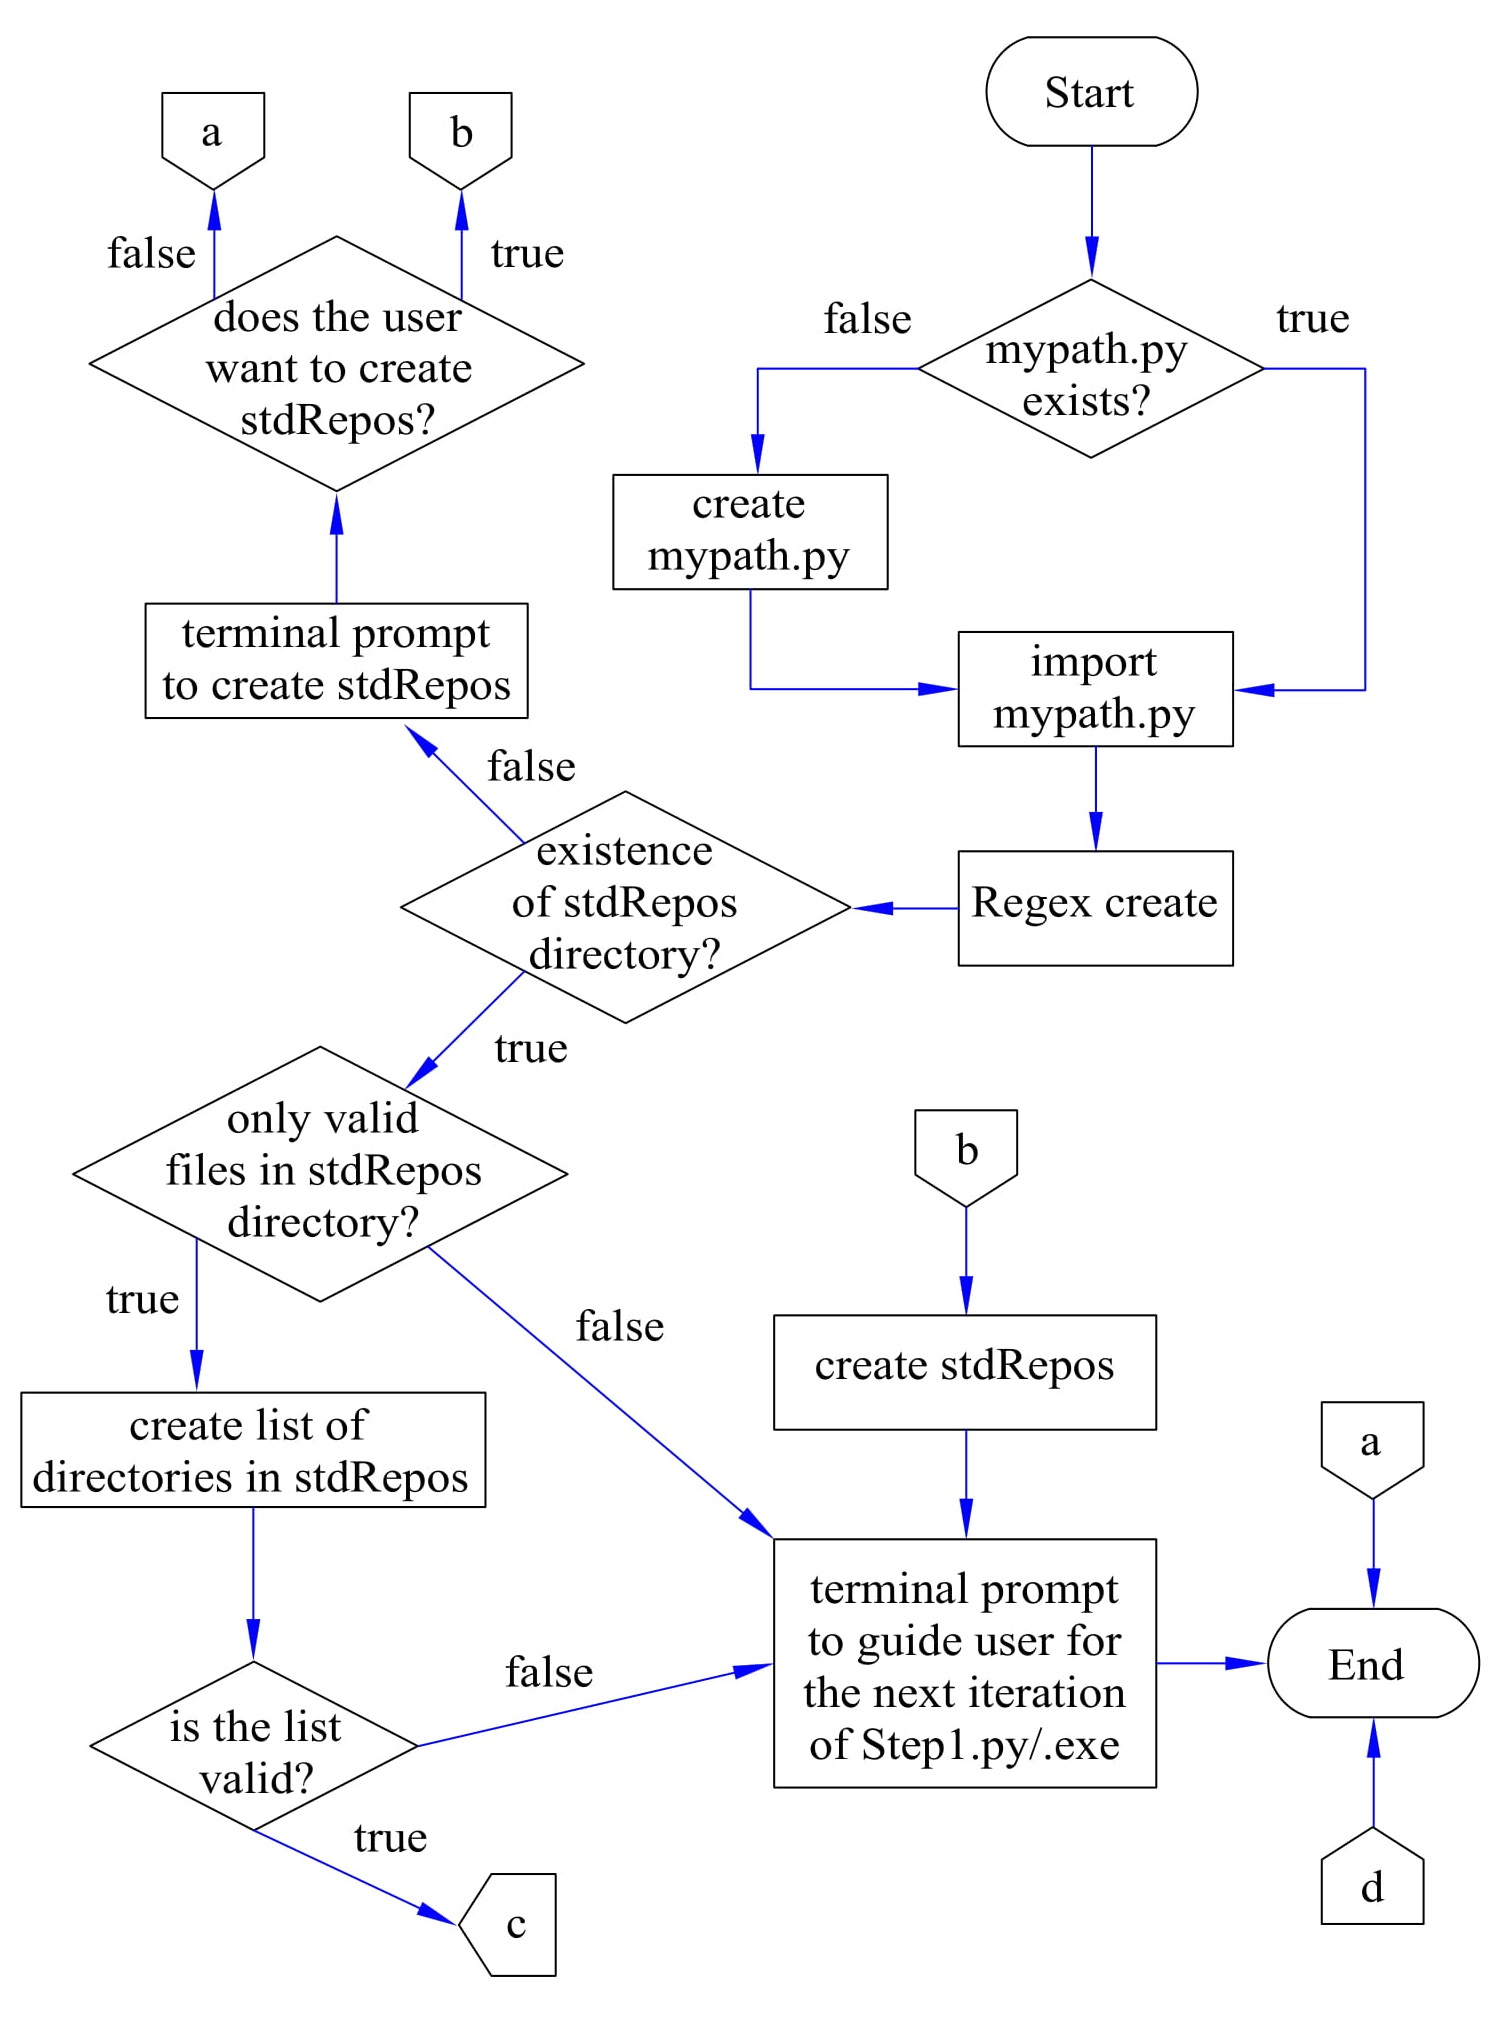
\includegraphics[width = 100mm]{1.1.jpg}
\caption{Step1 flow diagram 1}
\label{1.1}
\end{center}
\end{figure}

\begin{figure}[H]
\begin{center}
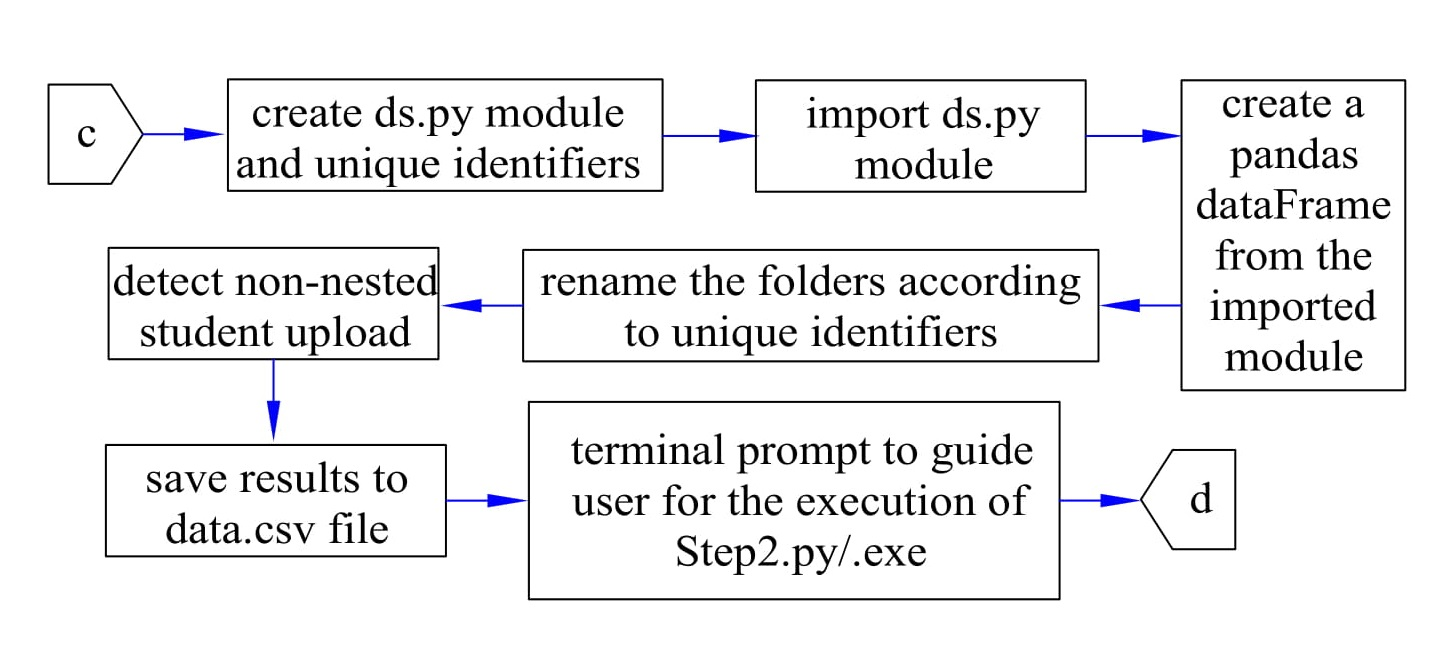
\includegraphics[width = 100mm]{1.2.jpg}
\caption{Step1 flow diagram 2}
\label{1.2}
\end{center}
\end{figure}

As can be see in Figure~\ref{1.1} and Figure~\ref{1.2}, the logical parts of the Step1.py/.exe are quite extensive and will only partially be discussed. 

\subsubsection{mypath.py module}
\label{mypath}

The various programs that comprise the autonomous system will be executed on a host PC other than the one they were created on. Since the user of the host PC can place the autonomous system (consisting of three programs) anywhere in the file system of the aforementioned PC, identifying the root repository becomes necessary. It is indeed important, that the programs in the autonomous chain, are able to execute regardless of where in the host file system they are located. 
\\\\
Regarding the above observation, it was decided that a python module is to be created in order to save the home, "stdRepos" and "data" directories. The code snippet below illustrates the process of creating the "data" directory as well as the mypath.py module. It further illustrates how the aforementioned module is imported into the program after creation.

\lstinputlisting[label={code1},caption={mypath.py and data folder creation and import}, language=Python]{code1.py}

It can be seen from Listing~\ref{code1}: lines 13 - 24 that the program will create a "data" directory within the home directory (where the programs are located). In addition to the creation of this directory, a module is created and stored within the "data" directory, namely mypath.py \cite{Sweigart2015}.
\\\\
It is of note, that the aforementioned functionality strictly occurs if the "data" directory and the mypath.py module does not yet exist. If these entities do however exist, the module is simply imported as per  Listing~\ref{code1}: lines 5 - 11. Since Step1.py/.exe is created with multiple executions in mind, the decision was taken to use the above approach.

\begin{figure}[H]
\begin{center}
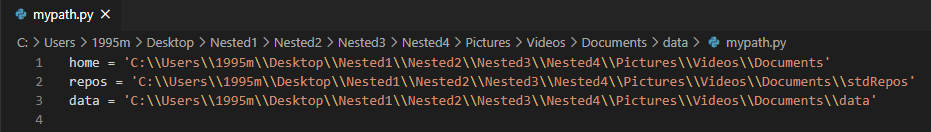
\includegraphics[width = 155mm]{mypath.pyCon.png}
\caption{mypath.py module content}
\label{mypath.pyCon}
\end{center}
\end{figure}

Figure~\ref{mypath.pyCon} illustrates the content of the pertaining module. Moreover, it illustrates how the directories of importance are stored regardless of location within a file system. The absolute path to the various directories are saved to be utilized by subsequent executions of Step1.py/.exe, in addition to the other programs in the autonomous chain.


\subsubsection{Regex creation}
\label{regex1}
As indicated in \textbf{\ref{p1} \nameref{p1}}, an important requisite of the autonomous process is the introduction of anonymity. It is, in fact, necessary to remove and replace all instances of student numbers from directory and file names. In order to facilitate the fulfilment of anonymity, it was decided to introduce regular expressions to the various programs in the autonomous system. These regular expressions are henceforth abbreviated simply as regex. 

\lstinputlisting[label={code2},caption={Step1 regex creation}, language=Python]{code2.py}

Listing~\ref{code2} depicts the regular expressions introduced as part of Step1.py/.exe. Lines 1-3 are simply regular expressions used to identify different variants of student numbers \cite{Sweigart2015}\cite{regex}. Line 4 consists of a regex pattern used to identify a validd unique identifier and will be expanded upon in \textbf{\nameref{stdRepos}}.
\subsubsection{stdRepos directory}
\label{stdRepos}
\lstinputlisting[label={code3},caption={Regex initialization}, language=Python]{code3.py}

Listing~\ref{code3} depicts the code written to:
\\
\begin{enumerate}
\item Detect the existence of the "stdRepos" directory.
\item Create the "stdRepos" directory if the user so wishes.
\item Detect valid repositories within the "stdRepos" directory.
\item Create and handle all command prompts associated with the above mentioned functionality.
\end{enumerate}

It can be seen from Listing~\ref{code3}: Lines 1-21, that the program will test for the existence of the "stdRepos" folder within the home directory. If this directory is not detected, a command prompt will be displayed giving the user the option to create the "stdRepos" folder in the correct location. Thereafter, the program will exist after prompting the user to rerun Step1.py/.exe.
\\\\
It is assumed that the user will extract any student repositories within the "stdRepos" folder. It can be seen from Listing~\ref{code3}: Line 24, that the regex mentioned in \textbf{\ref{regex1} \nameref{regex1}}, is applied to the directory names within the "stdRepos" folder. If a match is detected the matched string is appended to a list. This list will be used in future functional blocks. 
\\\\
It can, lastly, be seen that any invalid files in the "stdRepos" folder will also be detected by the program. If indeed a folder/file is located within the directory but is not matched by a student number detection regex or a unique identifier regex, a command prompt will guide the user in the next step. The aforementioned functionality is depicted in Listing~\ref{code3}: Lines 27-40.

\subsubsection{ds.py module}
\label{ds}
\begin{figure}[H]
\begin{center}
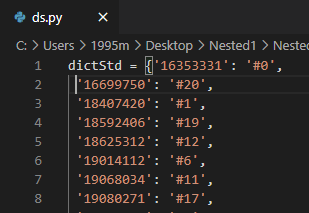
\includegraphics[width = 50mm]{ds.py.png}
\caption{ds.py module content}
\label{ds.pyCon}
\end{center}
\end{figure}

Figure~\ref{ds.pyCon} displays the content of the ds.py module. It depicts the linking of unique identifiers with student numbers. It is important to note that anonymity is not compromised by the ds.py module as it is deleted after the autonomous process finishes. Furthermore, each iteration of Step1.py/.exe randomly assigns unique identifiers to student numbers and the identifiers depicted in Figure~\ref{ds.pyCon}, will change from iteration to iteration. 

\lstinputlisting[label={code4},caption={ds.py creation}, language=Python]{code4.py}

Listing~\ref{code4}: Lines 1-12 depicts the code written to create a dictionary based on the content of the "stdRepos" folder. Randomly produced indexes are linked to student numbers and stored in a dictionary. It furthermore, illustrates (lines 14-24) how the mentioned dictionary is stored as a python module to be imported and utilized by the other steps in the autonomous process. 

\subsubsection{Pandas Data Frame}
\label{datFra}
It was decided to use a Pandas Data Frame to store any information extracted from student repositories. A Pandas Data Frame was selected above similar frameworks due to the ease with which data in the frame can be manipulated and searched. In order to populate the Pandas Data Frame, the previously created ds.py module must be imported by the program. This is all done in a very straight forward and standard way and will thus not be expanded upon.  


\subsubsection{Rename the folders}
\label{renFol}
\lstinputlisting[label={code5},caption={Folder renaming}, language=Python]{code5.py}

In Listing~\ref{code5}: lines 1-12, it can be observed that the folders within the "stdRepos" directory are renamed using a nested for-loop. The first for-loop iterates through all the folders within the "stdRepos" directory. The second (nested) for-loop, loops through the Pandas Data Frame (populated with unique identifiers linked to student numbers) and renames the current folder (the subject of the first for-loop) to the linked unique identifier.
\\\\
In short, for each folder in the "stdRepos" directory the Pandas Data Frame is looped to find the specific unique identifier associated with the pertaining folder student number. The folders are then renamed according to the identifier. 
\\
\subsubsection{data.csv file}
\label{data.csv}
Lastly, the previously mentioned Pandas Data Frame is stored as data.csv in the "data" directory. This file (data.csv) will be used to facilitate the population of Pandas Data Frames used by the subsequent steps in the automation process. 


\subsection{Step2.py}
\label{step2}

The figure below depicts the logical flow of the second python program as discussed and depicted in \textbf{\ref{p2} \nameref{p2}}. 

\begin{figure}[H]
\begin{center}
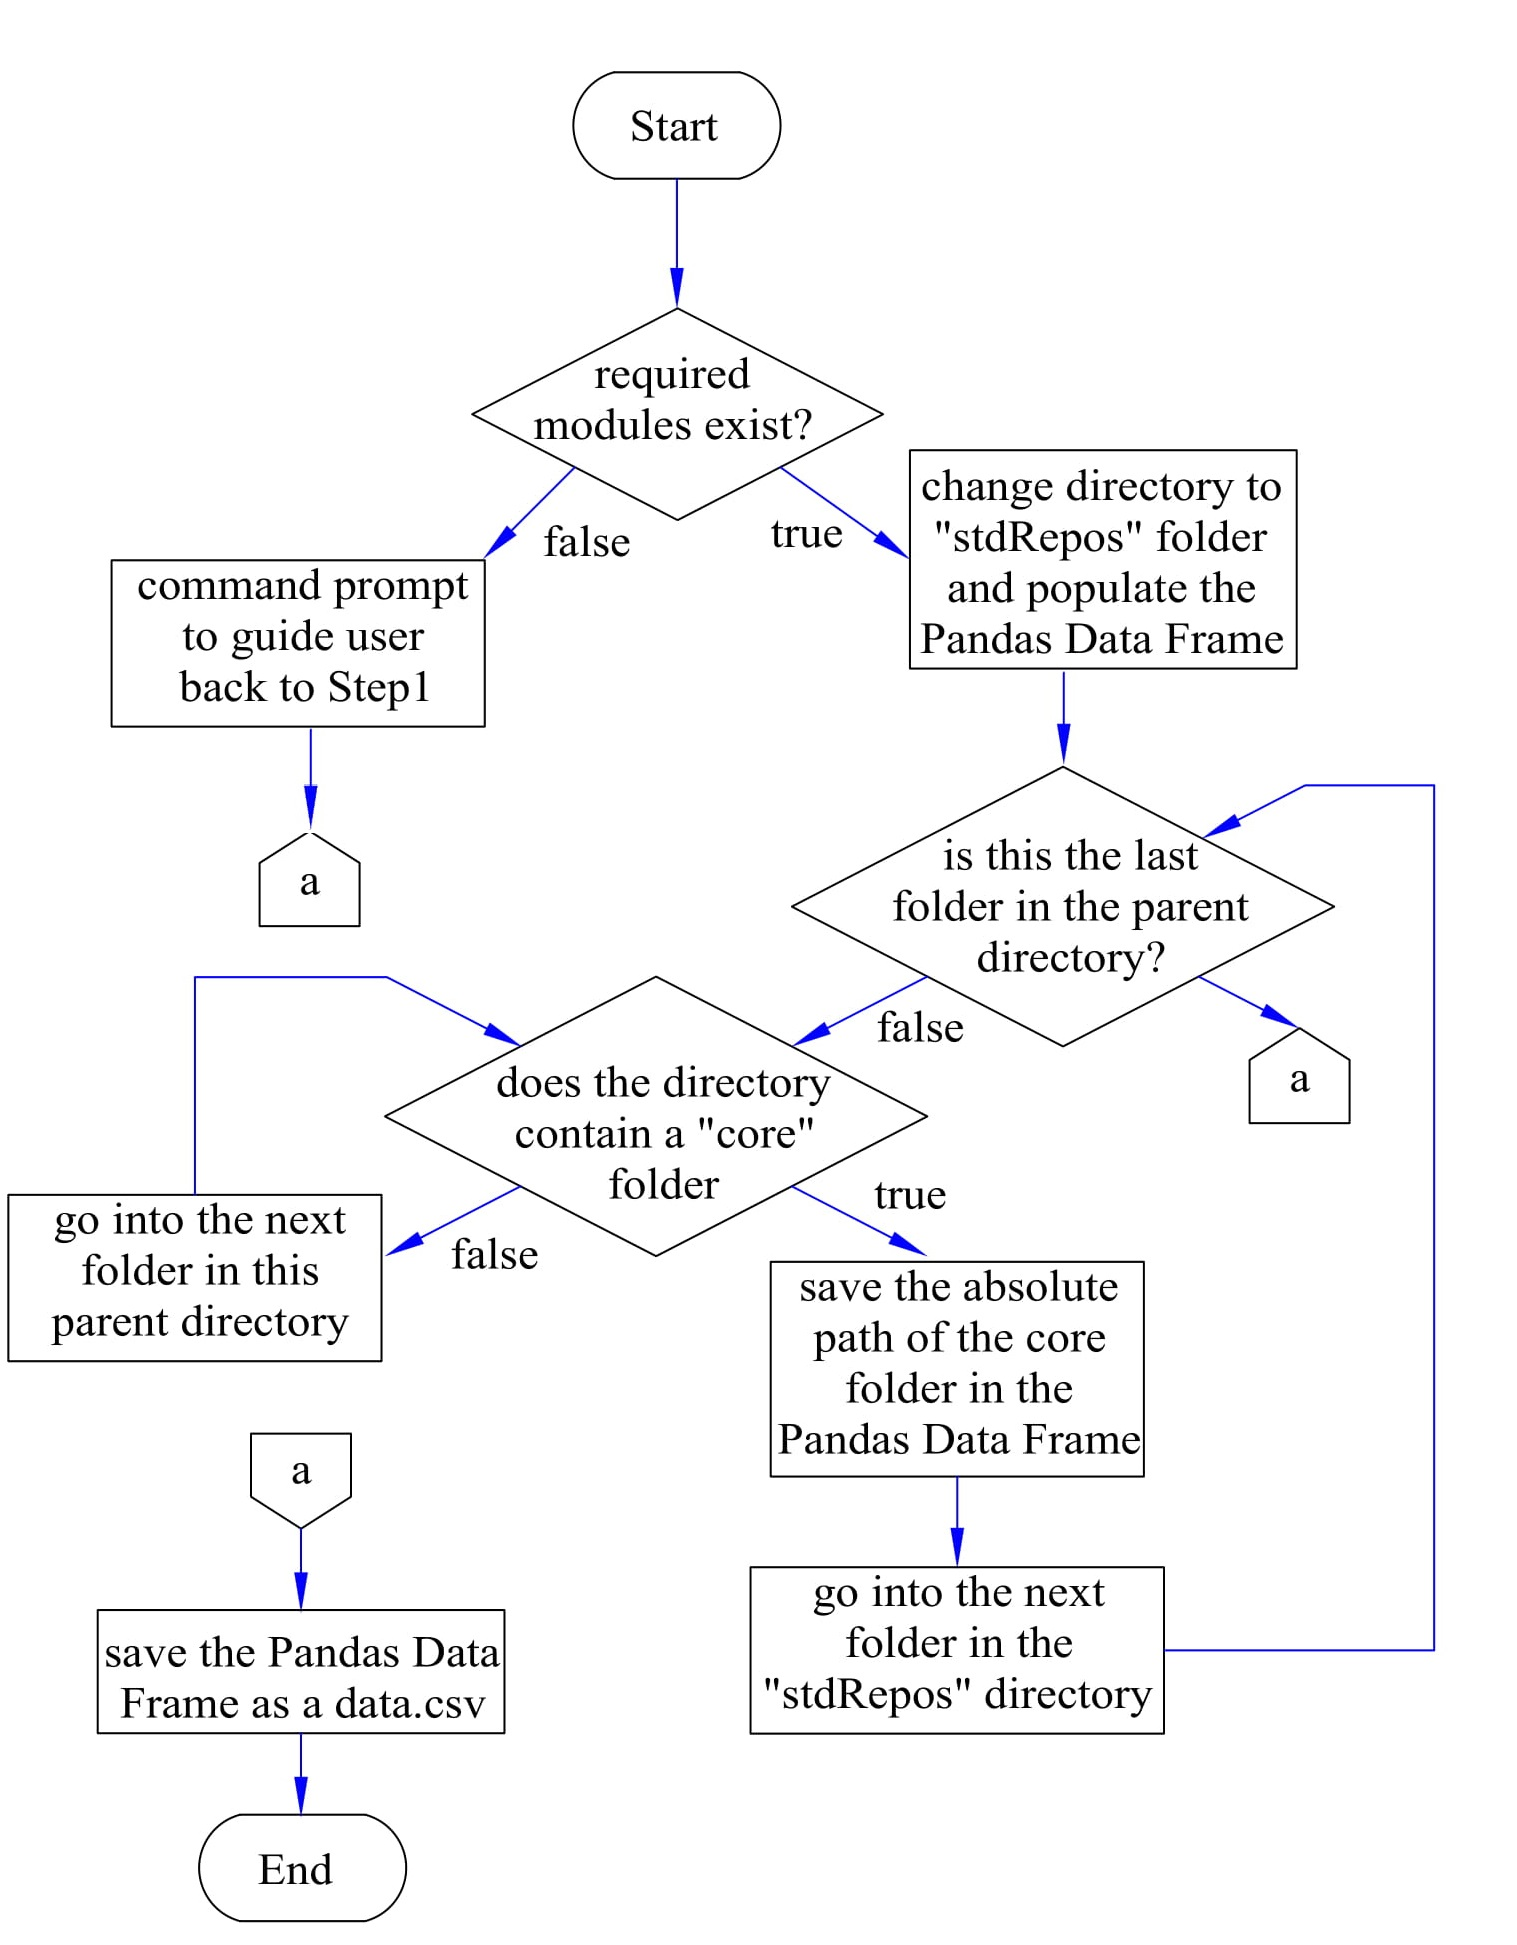
\includegraphics[width = 105mm]{2.jpg}
\caption{Step2 flow diagram}
\label{2}
\end{center}
\end{figure}

As can be see in Figure~\ref{2}, the logical parts of the Step2.py/.exe are recursive in nature and will be discussed in detail in the following subsections.

\subsubsection{Import the required modules}
\label{impMod}
It was shown in \textbf{\ref{step1} \nameref{step1}}, that various outputs are created and stored in the "data" directory. The outputs of importance are the mypath.py module as well as the data.csv file.
\\\\
In order for Step2.py/.exe to function as required, these two files need to be accessed by the program. This is done in a very simple way and will not be discussed in detail so as to remain succinct. In \textbf{\nameref{D}}, the code required for the importing of these files can be found. It is of note that a command prompt is created in case these modules are not found guiding the user back to Step1.py/.exe.
\\\\
Once the required modules are imported, mypath.py will be used - by the program in discussion - to navigate the various directories within the host PC file system. Additionally, the data.csv file will be used by the program to populate a Pandas Data Frame.

\subsubsection{Recurring function to identify the "core" directory}
\label{recFun}
The logical steps required by the program in discussion (Step2.py/.exe), is well suited to recurring function calls. This is because folders within the host PC must be navigated into and out of multiple times. This is indeed illustrated by Figure~\ref{2}. The goal of the pertaining program is to identify the "Core" directory within student repositories, as this directory contains the C code needed for evaluation. A problem requiring a novel solution however exists: Students often upload their repositories in such a way that the project directory is multiply nested. The solution to this problem can now be assessed. 

\lstinputlisting[label={code6},caption={Recurring function}, language=Python]{code6.py}

Listing~\ref{code6}: lines 1-12 illustrate the function used to identify and save the absolute path to the "Core" folder. Line 14 is the starting point of the folder navigation process and changes the directory to point to "stdRepos".
\\\\
The function begins by assessing the first folder in the parent directory. For the sake of explanation, this should be assumed to be the first student upload in the "stdRepos" folder. In line 3, it can be seen that the content of this folder (the first student upload) will be looped through. For each file/folder within this parent directory, an absolute path will be created as seen in line 4. Next, in lines 5-11, it will be determined whether or not the current folder within the parent directory is the "Core" folder. Line 5 serves simply to increase the speed of the function by preventing the program from navigating to a nested folder that is not of importance. It can be seen in line 7, that if indeed the "Core" folder is found within the parent directory, the absolute path to this folder will be saved into the Pandas Data Frame for the specific unique identifier associated with the student repository upload. Line 9 serves to prevent the program from attempting to navigate to a file that is not a directory. Finally it can be seen in lines 11 - 12, that folders other than "Core" will be navigated into by calling the core identification function (findCore) again and passing to it the absolute path of the nested folder.
\\\\
By making use of the above described recurring function paradigm, the "Core" folder to any student upload can be identified and saved for use by Step3.py/.exe regardless of projects nested within other folders.
\\\\
Lastly, the content of the Pandas Data Frame (now critically containing the path to the "Core" folder) is once again saved to data.csv in the "data" directory.

\newpage\cleardoublepage

\subsection{Step3.py}
\label{step3}

The figure below depicts the logical flow of the third python program as discussed and depicted in \textbf{\ref{p3} \nameref{p3}}. 

\begin{figure}[H]
\begin{center}
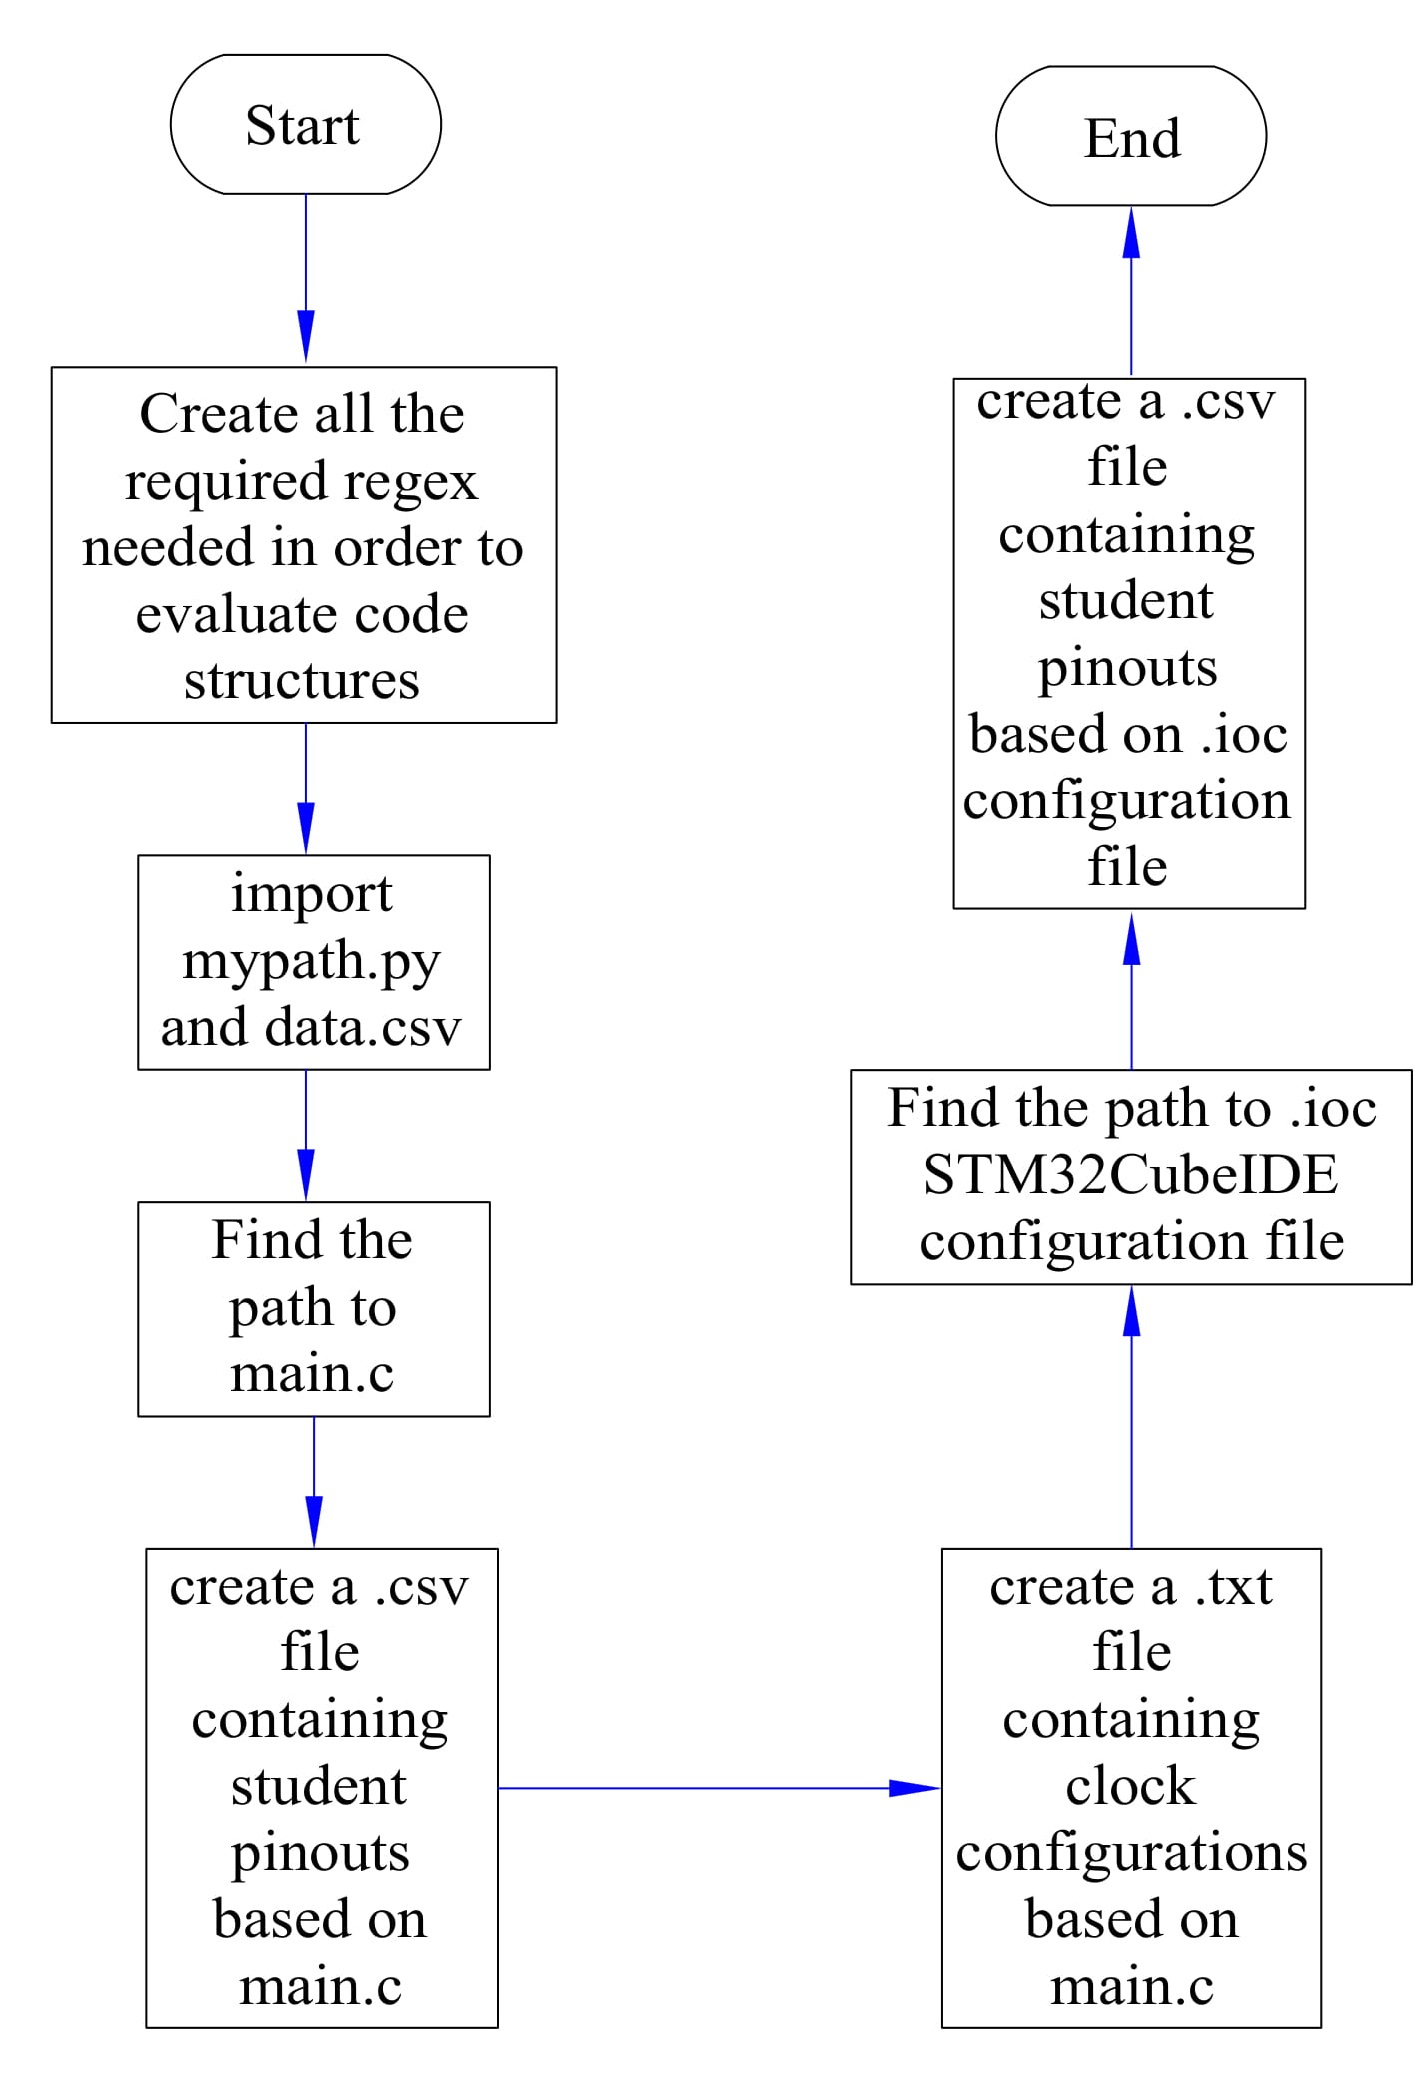
\includegraphics[width = 90mm]{3.jpg}
\caption{Step3 flow diagram}
\label{3}
\end{center}
\end{figure}

As can be seen in Figure~\ref{3}, the logical parts of the Step3.py/.exe are linear in execution. It is of note, that most of the autonomous process functionality has been handled by Step1.py/.exe and Step2.py/.exe. Step3.py/.exe simply produces the results.

\subsubsection{Regex creation}
\label{regCre}
Since Step3.py/.exe aims to extract information from student code for evaluation, it relies heavily on accurate and extensive regular expressions. The creation of these regular expressions are henceforth discussed:

\lstinputlisting[label={code7},caption={Step3 regex creation}, language=Python]{code7.py}

Listing~\ref{code7} depicts the regular expressions used in Step3.py/.exe. As can be seen, these regular expressions are quite extensive and will be discussed respectively. In line 1, a regular expression is created for the detection of the STM32CubeIDE created configuration file. Line 2 comprises the creation of a regular expression, used to identify pin configurations, within the STM32CubeIDE created configuration file. Next, line 3 details the creation of a regular expression used to identify clock configurations within the student produced main.c file. Lastly, lines 4 - 35 depict the regular expressions used to assess the pin configurations within the student created main.c file. 
\\\\
The two logical blocks in the flow diagram succeeding the creation of the regular expressions, are not discussed, but can be viewed in \textbf{\nameref{E}}

\subsubsection{Pin configuration file based on main.c}
\label{pinConMain.c}
\lstinputlisting[label={code8},caption={Pin configuration file based on main.c}, language=Python]{code8.py}

Listing~\ref{code8} depicts the process by which .csv files are created containing all the pin configurations of individual student MCU project uploads. Firstly, a Pandas Data Frame is created with columns according to the possible pin configuration options. In lines 3 - 9, the main.c file associated with a specific student repository is read. Additionally, exception handling is introduced for uploads that do not contain the required file. Lines 10 - 14 create empty lists, which are used to asses whether or not a specific line in main.c is indeed a pin configuration line. Next, lines 16 - 43 assess (using the regular expression described in the previous subsection) which pins are used by the student and how these pins are configured. Lastly, the result of the depicted code is stored as a .csv file using a unique identifier within the "data" folder.
\\
\subsubsection{Clock configuration file based on main.c}
\label{cloConMain.c}
\lstinputlisting[label={code9},caption={Clock configuration file based on main.c}, language=Python]{code9.py}

It can be seen in Listing~\ref{code9}, that all clock configuration lines within main.c are stored in a similar way to the method discussed in the preceding subsection. To avoid repetition, the logic of the depicted function will not be discussed excessively. Lines 5 - 14 loop through the content of main.c and store clock configurations (based on the regex discussed previously) in a .txt file within the "data" directory.
\\
\subsubsection{Pin configuration file based on .ioc}
\label{cloConMain.c}
\lstinputlisting[label={code10},caption={Pin configuration file based on .ico}, language=Python]{code10.py}

Listing~\ref{code10} shows how, in a manner similar to the aforementioned functions, pin configurations (based on the STM32CubeIDE .ioc configuration) file are saved. These pin configurations are also saved as .csv files and should be reconcilable with the configurations saved using the main.c file.
\\
\section{Windows executable files}
\label{exe}
It was mentioned in \textbf{\ref{scOfWrk} \nameref{scOfWrk}}, that the autonomous process was created with Windows PCs in mind. Due to this constraint, it becomes possible to create .exe versions of the three python programs. This enables any Windows PC to make use of the autonomous system without having to take python dependencies into account.
\\\\
This was done using pyinstaller, since it bundles all dependencies into a single .exe file which can simply be double clicked by the user of the host PC. It is important to note that a trade-off exists, when introducing this simplification: The single .exe files take much longer to execute than their python script counter parts.
